% The key schedule of SPARX-128/256

\begin{figure}
    \begin{center}
        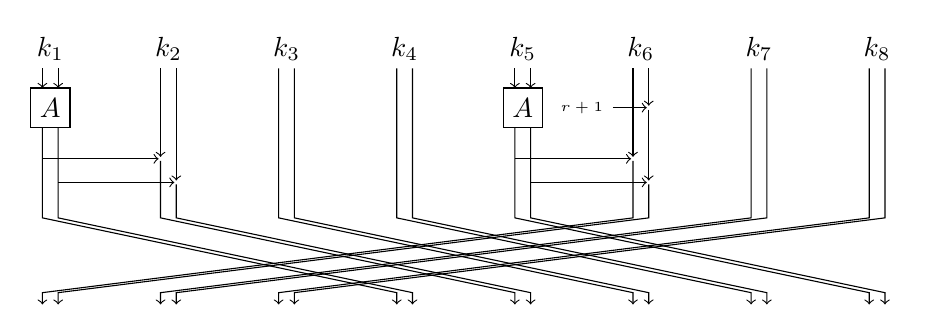
\begin{tikzpicture}[scale=0.5]
            %% input
            \draw (-10.5, +5.0) node(x0){$k_1$} ;
            \draw (-7.5, +5.0) node(x1){$k_2$} ;
            \draw (-4.5, +5.0) node(x0){$k_3$} ;
            \draw (-1.5, +5.0) node(x1){$k_4$} ;
            \draw (+1.5, +5.0) node(x2){$k_5$} ;
            \draw (+4.5, +5.0) node(x3){$k_6$} ;
            \draw (+7.5, +5.0) node(x2){$k_7$} ;
            \draw (+10.5, +5.0) node(x3){$k_8$} ;
            \draw[->] (-10.7, +4.5) -- (-10.7, +4.0) ;
            \draw[->] (-10.3, +4.5) -- (-10.3, +4.0) ;
            \draw[->] (+1.3, +4.5) -- (+1.3, +4.0) ;
            \draw[->] (+1.7, +4.5) -- (+1.7, +4.0) ;
            %% S-Box layer
            \draw (-11.0, +3.0) rectangle node[pos=0.5]{$A$} (-10.0, +4.0) ;
            \draw (+1.0, +3.0) rectangle node[pos=0.5]{$A$} (+2.0, +4.0) ;
            %% additions
            \draw (-7.7, +2.2) node[inner sep=0](add0){$\boxplus$} ;
            \draw (-7.3, +1.6) node[inner sep=0](add1){$\boxplus$} ;
            \draw[->] (-10.7, +2.2) -- (add0) ;
            \draw[->] (-10.3, +1.6) -- (add1) ;
            \draw (+4.3, +2.2) node[inner sep=0](add2){$\boxplus$} ;
            \draw (+4.7, +1.6) node[inner sep=0](add3){$\boxplus$} ;
            \draw[->] (+1.3, +2.2) -- (add2) ;
            \draw[->] (+1.7, +1.6) -- (add3) ;
            \draw (+4.7, +3.5) node[inner sep=0](addC){$\boxplus$} ;
            \draw (+3.0, +3.5) node(C){\tiny $r+1$} ;
            \draw[->] (C) -- (addC) ;
            % Data path
            \draw[->] (-10.7, 3.0) -- (-10.7, 0.7) -- (-1.7, -1.2) -- (-1.7, -1.5) ;
            \draw[->] (-10.3, 3.0) -- (-10.3, 0.7) -- (-1.3, -1.2) -- (-1.3, -1.5) ;
            \draw[->] (-7.7, 4.5) -- (add0);
            \draw[->] (add0) -- (-7.7, 0.7) -- (+1.3, -1.2) -- (+1.3, -1.5) ;
            \draw[->] (-7.3, 4.5) -- (add1) ;
            \draw[->] (add1) -- (-7.3, 0.7) -- (+1.7, -1.2) -- (+1.7, -1.5) ;
            \draw[->] (-4.7, 4.5) -- (-4.7, 0.7) -- (+4.3, -1.2) -- (+4.3, -1.5) ;
            \draw[->] (-4.3, 4.5) -- (-4.3, 0.7) -- (+4.7, -1.2) -- (+4.7, -1.5) ;
            \draw[->] (-1.7, 4.5) -- (-1.7, 0.7) -- (+7.3, -1.2) -- (+7.3, -1.5) ;
            \draw[->] (-1.3, 4.5) -- (-1.3, 0.7) -- (+7.7, -1.2) -- (+7.7, -1.5) ;
            \draw[->] (+1.3, 3.0) -- (+1.3, 0.7) -- (+10.3, -1.2) -- (+10.3, -1.5) ;
            \draw[->] (+1.7, 3.0) -- (+1.7, 0.7) -- (+10.7, -1.2) -- (+10.7, -1.5) ;
            \draw[->] (+4.3, 4.5) -- (add2) ;
            \draw[->] (add2) -- (+4.3, 0.7) -- (-10.7, -1.2) -- (-10.7, -1.5) ;
            \draw[->] (+4.7, 4.5) -- (addC) ;
            \draw[->] (addC) -- (add3) ;
            \draw[->] (add3) -- (+4.7, 0.7) -- (-10.3, -1.2) -- (-10.3, -1.5) ;
            \draw[->] (+7.3, 4.5) -- (+7.3, 0.7) -- (-7.7, -1.2) -- (-7.7, -1.5) ;
            \draw[->] (+7.7, 4.5) -- (+7.7, 0.7) -- (-7.3, -1.2) -- (-7.3, -1.5) ;
            \draw[->] (+10.3, 4.5) -- (+10.3, 0.7) -- (-4.7, -1.2) -- (-4.7, -1.5) ;
            \draw[->] (+10.7, 4.5) -- (+10.7, 0.7) -- (-4.3, -1.2) -- (-4.3, -1.5) ;
        \end{tikzpicture}
        \FigDef{sparx128ks256}{The 256-bit permutation $K_{8}^{256}$ used in \spnARXinstance{128}{256}.}
    \end{center}
\end{figure}


\begin{algorithm}
  \AlgDef{sparx128ks256}{\spnARXinstance{128}{256} key schedule permutation $K_{8}^{256}$.}
  \begin{algorithmic}
    \State{$r \gets r + 1$}
    \State{$k_1 \gets A(k_1)$}
    \State{$(k_2)_L \gets (k_2)_L + (k_1)_L \mod 2^{16}$}
    \State{$(k_2)_R \gets (k_2)_R + (k_1)_R \mod 2^{16}$}
    \State{$k_5 \gets A(k_5)$}
    \State{$(k_6)_L \gets (k_6)_L + (k_5)_L \mod 2^{16}$}
    \State{$(k_6)_R \gets (k_6)_R + (k_5)_R + r \mod 2^{16}$}
    \State{$k_1, k_2, k_3, k_4, k_5, k_6, k_7, k_8 \gets k_6, k_7, k_8, k_1, k_2, k_3, k_4, k_5$}
  \end{algorithmic}
\end{algorithm}
